\documentclass{article}
\usepackage{amsmath}
\usepackage{tikz}

\begin{document}

\title{Forwardpropagation Beispiel}
\author{}
\date{}
\maketitle



Betrachte das folgende relativ einfache Beispiel: \\


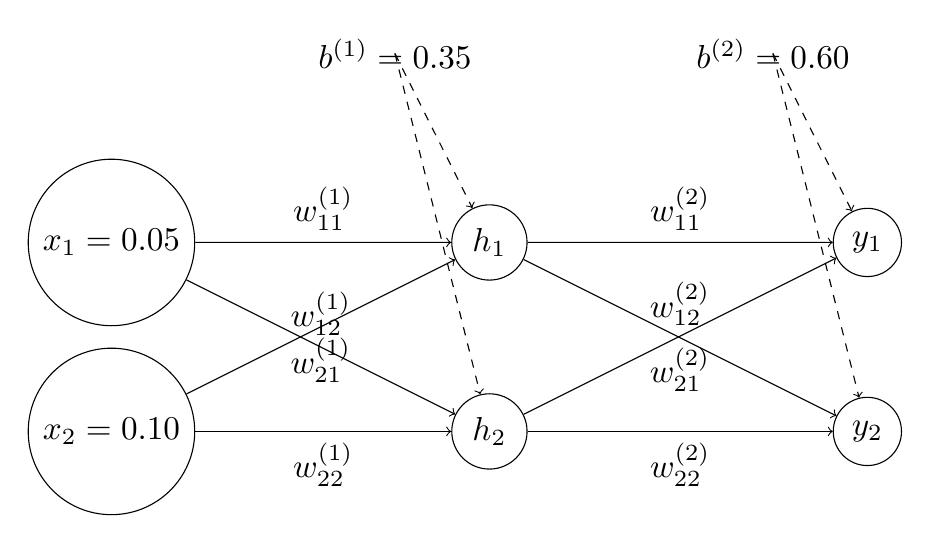
\begin{tikzpicture}[scale=1.2, transform shape]

% Input Layer
\node[draw, circle] (I1) at (0,2) {$x_1 = 0.05$};
\node[draw, circle] (I2) at (0,0) {$x_2 = 0.10$};

% Hidden Layer
\node[draw, circle] (H1) at (4,2) {$h_1$};
\node[draw, circle] (H2) at (4,0) {$h_2$};

% Output Layer
\node[draw, circle] (O1) at (8,2) {$y_1$};
\node[draw, circle] (O2) at (8,0) {$y_2$};

% Input to Hidden Layer Weights
\draw[->] (I1) -- (H1) node[midway, above] {$w^{(1)}_{11} $};
\draw[->] (I1) -- (H2) node[midway, above] {$w^{(1)}_{12} $};
\draw[->] (I2) -- (H1) node[midway, below] {$w^{(1)}_{21} $};
\draw[->] (I2) -- (H2) node[midway, below] {$w^{(1)}_{22} $};

% Hidden to Output Layer Weights
\draw[->] (H1) -- (O1) node[midway, above] {$w^{(2)}_{11} $};
\draw[->] (H1) -- (O2) node[midway, above] {$w^{(2)}_{12} $};
\draw[->] (H2) -- (O1) node[midway, below] {$w^{(2)}_{21} $};
\draw[->] (H2) -- (O2) node[midway, below] {$w^{(2)}_{22} $};

% Biases as text only (no circles)
\node at (3, 4) {$b^{(1)} = 0.35$};
\node at (7, 4) {$b^{(2)} = 0.60$};

% Bias connections (dashed lines)
\draw[->, dashed] (3, 4) -- (H1);
\draw[->, dashed] (3, 4) -- (H2);
\draw[->, dashed] (7, 4) -- (O1);
\draw[->, dashed] (7, 4) -- (O2);

\end{tikzpicture}


\subsubsection*{Voraussetzungen des Beispiels:}

\begin{itemize}
    \item 2 Eingabeknoten: \( x_1 = 0.05 \), \( x_2 = 0.10 \)
    \item 2 versteckte Knoten: \( h_1, h_2 \)
    \item 2 Ausgabeknoten: \( y_1, y_2 \)
    \item Lernrate: \( \eta = 0.5 \)
\end{itemize}


\textbf{Gewichte und Biases:}
\[
W^{(1)} = \begin{pmatrix}  0.149658 & 0.2493165 \\ 0.19964325 & 0.2992865 \end{pmatrix}, \quad
b^{(1)} = \begin{pmatrix} 0.35 \\ 0.35 \end{pmatrix}
\]
\[
W^{(2)} = \begin{pmatrix} 0.359025 & 0.408785 \\ 0.511435 & 0.561495 \end{pmatrix}, \quad
b^{(2)} = \begin{pmatrix} 0.60 \\ 0.60 \end{pmatrix}
\]
%
\textbf{Zielausgaben:}
\[
y_{\text{target}, 1} = 0.01, \quad y_{\text{target}, 2} = 0.99
\]

\subsubsection*{Schritt 1: Vorwärtsdurchlauf}

1. Berechnung der Nettoeingänge für die versteckte Schicht:\\
\[
z^{(1)}_1 = x_1 \cdot w^{(1)}_{11} + x_2 \cdot w^{(1)}_{12} + b^{(1)}_1 = 0.05 \cdot 0.149658 + 0.10 \cdot 0.2493165 + 0.35 = 0.3824145
\]
\[
z^{(1)}_2 = x_1 \cdot w^{(1)}_{21} + x_2 \cdot w^{(1)}_{22} + b^{(1)}_2 = 0.05 \cdot 0.19964325 + 0.10 \cdot 0.29928650 + 0.35 = 0.3899108
\]
\\
%
2. Aktivierung der versteckten Knoten mit der Sigmoid-Funktion:
\[
h_1 = \sigma(z^{(1)}_1) = \frac{1}{1 + e^{-0.3824145}} = 0.594455
\]
\[
h_2 = \sigma(z^{(1)}_2) = \frac{1}{1 + e^{-0.3899108}} = 0.59626
\] \\
%
3. Berechnung der Nettoeingänge für die Ausgabeschicht:
\[
z^{(2)}_1 = h_1 \cdot w^{(2)}_{11} + h_2 \cdot w^{(2)}_{12} + b^{(2)}_1 = 0.594455 \cdot 0.359025 + 0.59626 \cdot 0.408785 + 0.60 = 1.05716
\]
\[
z^{(2)}_2 = h_1 \cdot w^{(2)}_{21} + h_2 \cdot w^{(2)}_{22} + b^{(2)}_2 = 0.594455 \cdot 0.511435 + 0.59626 \cdot 0.561495 + 0.60 = 1.23882
\]\\
%
4. Aktivierung der Ausgabeknoten:
\[
y_1 = \sigma(z^{(2)}_1) = \frac{1}{1 + e^{-1.05716}} = 0.742147
\]
\[
y_2 = \sigma(z^{(2)}_2) = \frac{1}{1 + e^{-1.23882}} = 0.775358
\]
\\
\subsubsection*{Schritt 2: Fehlerberechnung (Loss)}
Verwende die Mean Squared Error (MSE) als Fehlerfunktion:
\[
L = \frac{1}{2} \left( (y_{\text{target},1} - y_1)^2 + (y_{\text{target},2} - y_2)^2 \right)
\]
\[
L = \frac{1}{2} \left( (0.01 - 0.742147)^2 + (0.99 - 0.775358)^2 \right) = \frac{1}{2} \left( 0.536039 +  0,046071 \right) = 0.291055
\]

\end{document}
